\section{Probabilistic Models}
Assuming $P(C_{1}) = \pi$, $P(x|C_{i})\nu (x; \N _{i}, \Sigma$). Given the dataset $D = {(x_{n}, t_{n})^{N}_{n=1}}, t_{n}=1$ if $x_{n}$ belongs to class $C_{1}$, $T_{n} = 0$ otherwise.

$N_{1}$ is the number of samples in D belonging to $C_{1}$ and $N_{2}$ be the number of samples from $C_{2}$ ($N = N_{1} + N_{2}$).

The likelihood function is:
\begin{equation}
    P(t|\pi, \mu _{1}, \mu_{2}, \Sigma, D) = \prod_{n=1}^{N}[\pi \N (x_{n};\mu_{1}, \Sigma)]^{t_{n}}
    [(1 - \pi) \N (x_{n};\mu_{2}, \Sigma)]^{(1 - t_{n})}
\end{equation}
Determine $\pi, \mu_{!}, \mu_{2}, \Sigma$

By maximizing the log likelihood function we obtain:
\begin{equation}
    \pi = \frac{N_{1}}{N}, \\
    \mu_{1} = \frac{1}{N_{1}} \sum_{n=1}^{N}t_{n}x_{n}, \\
    \mu_{2} = \frac{1}{N_{2}} \sum_{n=1}^{N}t_{n}x_{n}, \\
    \Sigma = \frac{N_1}{N}S_{1} + \frac{N_2}{N}S_{2}. 
\end{equation}
with $S_{i} = \frac{1}{N_{i}} \sum_{n \in C_{i}}(x_{n} - \mu_{i})(x_{n} - \mu_{i})^{T}$, $i = 1, 2$.

If we want to predict a new sample $x'$:
\begin{equation}
    P(C_{1}|x') = \sigma (w^{T}x' + W_{0})
\end{equation}
\subsection{Multiple classes}

\begin{equation}
    P(C_{k}|x) = \frac{P(x|C_{k})P(C_{k})}{\sum_{j}P(x|C_{j})P(C_{j})} = \frac{exp(a_{k})}{\sum_{j}exp(a_{j})}
\end{equation}
with $a_{k} = \ln P(x|C_{k})P(C_{k})$\ \

\subsection{Gaussian Naive Bayes}
$P(C_{k}) = \pi_{k}, P(x|C_{k}) = \N(x: \mu_{k}, \Sigma)$
Data set $D = \{(x_{n}, t_{n})^{N}_{n=1}\}$, with $t_{n}$ 1-of-K encoding
\begin{equation}
    \pi = \frac{N_{k}}{N}, \\
    \mu_{k} = \frac{1}{N_{k}} \sum_{n=1}^{N}t_{nk}x_{n}, \\
    \Sigma = \sum_{k=1}^{K}\frac{N_k}{N}S_{k}, 
    S_{k} = \frac{1}{N_{k}} \sum_{n = 1}^{N} t_{nk}(x_{n} - \mu_{k})(x_{n} - \mu_{k})^{T}
\end{equation}
Prediction of new sample $x \not\in D$
\begin{equation}
    \underset{C_{k} \in C}{argmax} P(C_{k}|x) = \underset{k}{argmax}\frac{exp(a_{k})}{\sum_{j}exp(a_{j})}
\end{equation}
with $a_{k} = \ln P(x|C_{k}) P(C_{k})$

\subsection{Compact Notation}
Model:
\begin{equation}
    w^{T}x + w_{0} = (w_{0} w)(
    \begin{bmatrix} 
        1 \\
        x
    \end{bmatrix})
\end{equation}

\section{Discriminative models}
In the discriminative models we only want to compute the posterior probabilities without estimating the distribution. We can not sample new elements from the distribution

The likelihood for a parametric model $M_{\Theta}: P(t|\Theta, D), D = $ and the maximum likelihood solution is:
\begin{equation}
    \Theta^{*} = \underset{\Theta}{argmax}\ln P(t|\Theta, X)
\end{equation}
when $M _\Theta$ belongs to the exponential family, likelihood $P(t|\Theta, X)$ can be expressed in the form $P(t|\Tilde{w}, X)$, with maximum likelihood
\begin{equation}
    \Tilde{w}^{*} = \underset{\Tilde{w}}{argmax} ln P(t|\Tilde{w}, X)
\end{equation}
Without estimating the model parameters. Simplified notation: $P(t|\Tilde{w})$

\subsection{Logistic regression}
\subsubsection{Two classes}
given the dataset $D$ with each sample of the dataset $t_{i} \in \{0, 1\}$

Likelihood function:
\begin{equation}
    p(t|\Tilde{w}) = \prod_{n=1}^{n} y^{t_{n}}_{n}(1 - y_{n})^{1 - t_{n}}
\end{equation}
with 
\[t_{n} = p(C_{1}|\Tilde{x}_{n}) = \sigma(\Tilde{w}^{T}\Tilde{x}_{n}) = \frac{1}{1 + e^{-\Tilde{w}^{T}\Tilde{x}_{n}}}\]

If we use the logarithm of the previous formula as loss function, we get the cross entropy error function (negative log likelihood)
\begin{equation}
    E(\Tilde{w}) \equiv -\ln P(t|\Tilde{w}) = -\sum^{N}_{n=1} [t_{n}\ln y_{n} + (1 - t_{n}) \ln (1 - y_{n})]
\end{equation}

We have to solve $\Tilde{w}^{*} = \underset{\Tilde{w}}{argmin}E(\Tilde{w})$. Many solvers are available for this problem.

\paragraph{Iterative reweight least squares}
Neqton-Raphson iterative optimization for minimizing the Gradient of the error wrt $\Tilde{w}$
\begin{equation}
    \nabla E(\Tilde{w}) = \sum_{n=1}^{N}(y_{n} - t_{n})\Tilde{x}_{n}
\end{equation}
Gradient descent step
\begin{equation}
    \Tilde{w} \xrightarrow[]{} \Tilde{w} - H(\Tilde{w})^{-1}\nabla E(\Tilde{w})
\end{equation}
where $H(\Tilde{w}) = \nabla \nabla E(\Tilde{w})$ is the Heissan matrix of $E(\Tilde{w})$

Classify a new sample $\Tilde{x}'$ as $C_{k}$ where $k^{*} = \underset{k=1\dots K}{argmax} P(C_{k}|\Tilde{x}', \Tilde{w}^{*})$

\paragraph{Generalization}
if we have a target function $f: X \xleftarrow{}C$ and a dataset $D$ we define an error function $E(\Theta)$ and solve the optimization problem
\begin{equation}
    \Theta^{*} = \underset{\Theta}{argmin} E(\Theta)
\end{equation}
and classify a new sample as $y(x'; \Theta^{*})$

\subsubsection{Learning in feature space}
we can replace $x_{n}$ with $\Phi(x_{n})$ to transform the dataset in an input space to get $\Phi'$ (we transform the dataset).

\paragraph{Compact notion}
two classes:
\begin{equation}
    y(x) = w^{T}x + w_{0} = \Tilde{w}^{T}\Tilde{x}
\end{equation}
with
\begin{equation}
    \Tilde{w} = \begin{bmatrix} 
                    w_{0} \\
                    w
                \end{bmatrix},
    \Tilde{x} = \begin{bmatrix} 
                    1 \\
                    x
                \end{bmatrix}
\end{equation}
with k classes there are more rows

\paragraph{Multiple classes}
Cannot use combination of binary linear models!!!
One-versus-the-rest classifiers and one-versus-one-classifiers. We can instead use K-class discriminant comprising K linear functions. Then classify x as $C_{k}$ if $y_{k}(x) > y_{j}(x)$ for all $j \neq k$. Decision boundary between $C_{k}$ and $C_{j}$:
\begin{equation}
    (\Tilde{w}_{k} - \Tilde{w}_{j})^{T}\Tilde{x} = 0
\end{equation}

\section{Learning linear discriminant}
methods to solve the linear discriminant problem
\subsection{Least Squares}
Given the dataset $D$, use 1 of K coding scheme, where each row is $t_{n} = (0, \dots, 1, \dots, 0)^{T}$

Minimize
\begin{equation}
    E(\Tilde{W}) = \frac{1}{2} \Tr{(\Tilde{X}\Tilde{W}\ T)^{T} ( \Tilde{X}\Tilde{W}\ T)}
\end{equation}
where:
\begin{equation}
    \Tilde{W} = (\Tilde{X}^T\Tilde{X})^{-1}(\Tilde{X}^{T}\ T)
\end{equation}
the $(\Tilde{X}^T\Tilde{X})^{-1}$ term is usually called pseudo inverse and is denoted as $X^{\dagger}$. Note: Least square is not robust to outliers.

\subsection{Perceptron}

\begin{figure}[H]
    \centering
    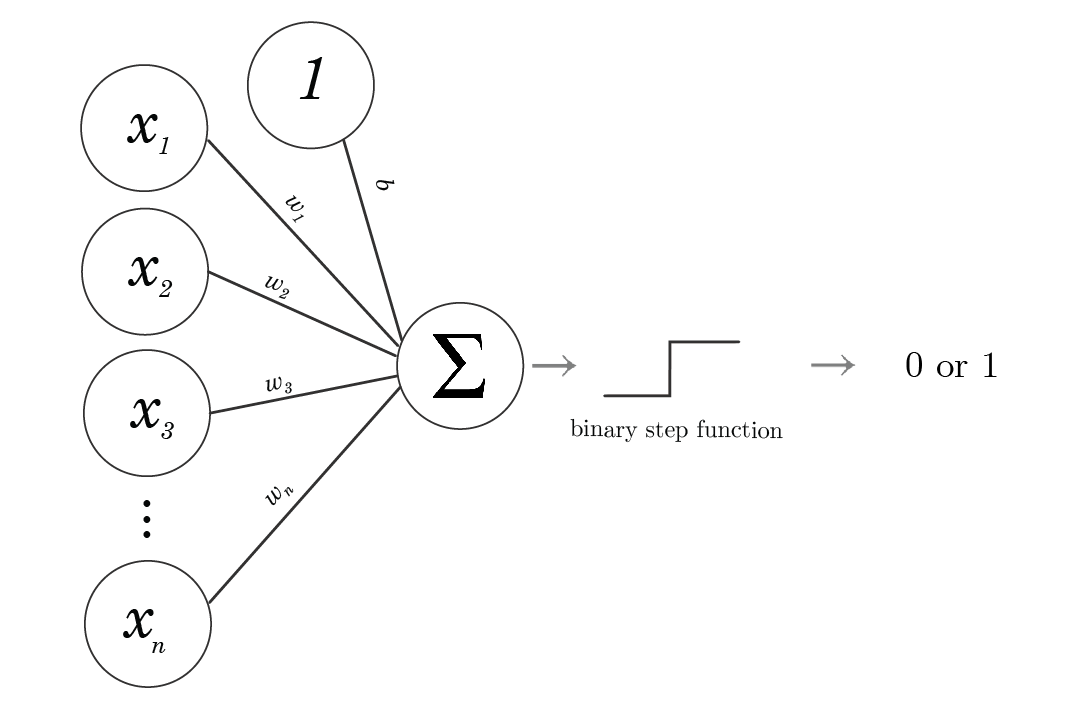
\includegraphics[width=15cm]{images/Probabilistic Models/perceptron.png}
    \caption{}
    \label{fig:perceptron}
\end{figure}

$o(x_{1}, \dots, x_{d})$ is 1 if $w_{0} + w_{1}x_{1} + \dots +w_{0} + w_{n}x_{n} > 0$, -1 otherwise.

The perceptron training rule is to minimize the squared error (loss function):
\begin{equation}
    E(w) \equiv \frac{1}{2}\sum_{n=1}^{N}(t_{n} - o_{n})^{2} = \frac{1}{2} \sum_{n=1}^{N}
(t_{n} - w^{T}x_{n})^2\end{equation}

if we calculate the derivative of the error function we get:
\begin{equation}
    \frac{\partial E}{\partial w_{i}} = \dots = \sum_{n=1}^{N}(t_{n} - w^{T}x_{n})(-x_{i,n})
\end{equation}

and then we use this derivative to move weights towards the the minimum.
\begin{equation}
    w_{i} \xleftarrow{} w_{i} + \eta \Delta w_{i}
\end{equation}
where $\Delta w_{i}$ is the derivative of the loss. 

Perceptron converge if training data is clearly separable and the learning rate $\eta$ is sufficiently small.
It can terminate if the error reaches a threshold or there is a max number of iterations.

\subsection{Ficher's linear discriminant}
adjust w to find a direction that maximizes class separation based on the projection on the line. Consider a data set with $N_{1}$ points in $C_{1}$ and $N_{2}$ points in $C_{2}$
\begin{equation}
    m1 = \frac{1}{N_{1}}\sum_{n \in C_{1}}x_{n}
\end{equation}
\begin{equation}
    m2 = \frac{1}{N_{2}}\sum_{n \in C_{2}}x_{n}
\end{equation}
choose w that maximizes $J(w) = w^{t}(m_{2} - m_{1})$, subject to $||w|| = 1$
\begin{equation}
    w \propto S^{-1}_{W}(m_{2} - m_{1})
\end{equation}

we have to maximize 
\begin{equation}
    J(w) = \frac{w^{T}S_{B}w}{w^{T}S_{W}w}
\end{equation}
by solving $\frac{d}{dw}J(w) = 0$. In this formula, $S_{B}$ is the between covariance matrix while $S_{w}$ is the within covariance matrix.

\subsection{Support Vector Machines}
Support Vector Machines (SVM) for classification aims at finding a maximizing the margin providing better accuracy.

Assume that the dataset is linearly separable,

let $x_{k}$ be the closest point of the data set $D$ to the hyperplane $\overline{h}: \overline{w}^{T}x + \overline{w_{0}}$.
The \textbf{margin} (smallest distance between $x_{k}$ and $\overline{h}$) is $\frac{y(x_{k}}{||w||}$
So, given a dataset, the margin is computed as: 
\begin{equation}
    \underset{n=1, \dots , N}{min} \frac{y(x_{k})}{||w||} = \dots = \frac{1}{||w||} \underset{n=1, \dots , N}{min} [t_{n}(\overline{w}^{T}x_{n} + \overline{w_{0}})]
\end{equation}
using the property $|y(x_{n})| = t_{n}y(x_{n})$

Now we can calculate the hyperplane with the maximum margin by maximizing:
\begin{equation}
    w^{*}, w_{0}^{*} = \underset{w, w_{0}}{argmax} \frac{1}{||w||} \underset{n=1, \dots , N}{min} [t_{n}(w^{T}x_{n} + w_{0})]
\end{equation}
We can rescale the dataset such that the closest point $x_{k}$ has:
\begin{equation}
    t_{k}(w^{T}x_{k} + w_{0}) = 1
\end{equation}
and each other point has margin $\geq 1$

When we find the maximum margin hyperplane $w^{*}, w_{0}^{*}$, there will be at least 2 closest points $x_{k}^{\oplus}$ and $x_{k}^{\ominus}$ (one for each class).
The margin for $x_{k}^{\oplus}$ will be +1 while the margin for $x_{k}^{\ominus}$ will be -1.

In order to find a solution to he problem:
\begin{equation}
    w^{*}, w_{0}^{*} = argmax \frac{1}{||w||} = argmin \frac{1}{2} ||w||^{2}
\end{equation}
subject to:
\begin{equation}
    t_{n}(w^{T}x_{n} + w_{0}) \geq 1 \forall n = 1, \dots, N
\end{equation}
we can use the quadratic programming solution with the Lagrangian method.
The solution will be:
\begin{equation}
    w^{*} = \sum_{n=1}^{N} a_{n}^{*}t_{n}x_{n}
\end{equation}
$a_{i}^{*}$ (Lagrange multipliers): result of the Lagrangian optimization problem:
\begin{equation}
    \Tilde{L}(a) = \sum_{n=1}^{N}a_{n} - \frac{1}{2} \sum_{n=1}^{N}\sum_{m=1}^{N}a_{n}a_{m}t_{n}t_{m}x_{n}^{T}x_{m}
\end{equation}
subject to
\begin{equation}
    \begin{multlined}
        a_{n} \geq 0 \ \forall n = 1, \dots, N \\
        \sum_{n=1}^{N}a_{n}t_{n} = 0
    \end{multlined}
\end{equation}

\paragraph{Notes}
samples $x_{n}$ for which $a_{n}^{*} = 0$ will not count to the solution. \\
Karush-Kuhn-Tucker (KKT) condition:
for each $x_{n} \in D$, either $a_{n}^{*} = 0$ or $t_{n}y(x_{n}) = 1$ \\
thus $t_{n}y(x_{n}) > 1$ implies $a_{n}^{*} = 0$ \\
Support vectors are those points such that $t_{k}y(x_{k}) = 1$ and $a_{k}^{*} > 0$
\begin{equation}
    SV \equiv \{x_{k} \in D | t_{k}y(x_{k}) = 1\}
\end{equation}

If we want to express the hyperplane with his support vectors we can use:
\begin{equation}
    y(x) = \sum_{x_{j} \in SV}a_{j}^{*}t_{j}x^{T}x_{j}\text{ è }w_{0}^{*} = 0
\end{equation}

To compute $w_{0}^{*}$, we have to find support vectors that satisfies $t_{k}y(x_{k}) = 1$:
\begin{equation}
    t_{k}(\sum_{x_{j} \in SV}a_{j}^{*}t_{j}x_{k}^{T}x_{j}) = 1
\end{equation}
multiplying by $t_{k}$ and using $t_{k}^{2} = 1$ 
\begin{equation}
    w_{0}^{*} = t_{k} - \sum_{x_{j} \in SV}a_{j}^{*}t_{j}x_{k}^{T}x_{j}
\end{equation}

Instead of using one particular support vector $x_{k}$ to determine $w_{0}$, a more stable solution can be obtained by averaging over all the support vectors:
\begin{equation}
    w_{0}^{*} = \frac{1}{|SV|}\sum_{x_{k} \in SV}\left(t_{k} - \sum_{x_{j} \in S} a_{j}^{*}t_{j}x_{k}^{T}x_{j}\right)
\end{equation}

In order to classify a new instance, we can look at the sign:
\begin{equation}
    y(x') = sign\left(\sum_{x_{k} \in SV} a_{j}^{*}t_{j}x'^{T}x_{j}\right)
\end{equation}

\paragraph{Soft margin}
If data is almost linearly separable, we can use a soft margin $\xi _{n} \geq 0,\ n=1, \dots, N$ (called slack variable).
A soft margin lets some of the points to lay between the support vectors, adding a border.
\begin{equation}
    \begin{multlined}
        t_{n}y(x_{n}) \geq 1 - \xi _{n}, \ n=[1, \dots, N] \\
        w^{*}, w_{0}^{*} = \argmin \frac{1}{2} ||w||^{2} + C\sum_{n=1}^{N}\xi_n{} \\
        subject\ to\\
        t_{n}y(x_{n}) \geq 1 - \xi_{n}, \ n=1, \dots, N\\
        \xi_{n} \geq 0, n=1, \dots, N
    \end{multlined}
\end{equation}
where $C$ is a constant.

\subsection{Basis Function}
Until now, we considered only models that work directly on the dataset $D$, but what if we first perform a non-linear transformation of the inputs $\Phi  (x)$ (basis function)?.\\
By transforming the data, we can then find a linear hyperplane for the feature space $\Phi (D)$ that is not linear in the original space of $D$, actually separating points that were not linearly separable before the transformation.


\begin{figure}[H]
    \centering
    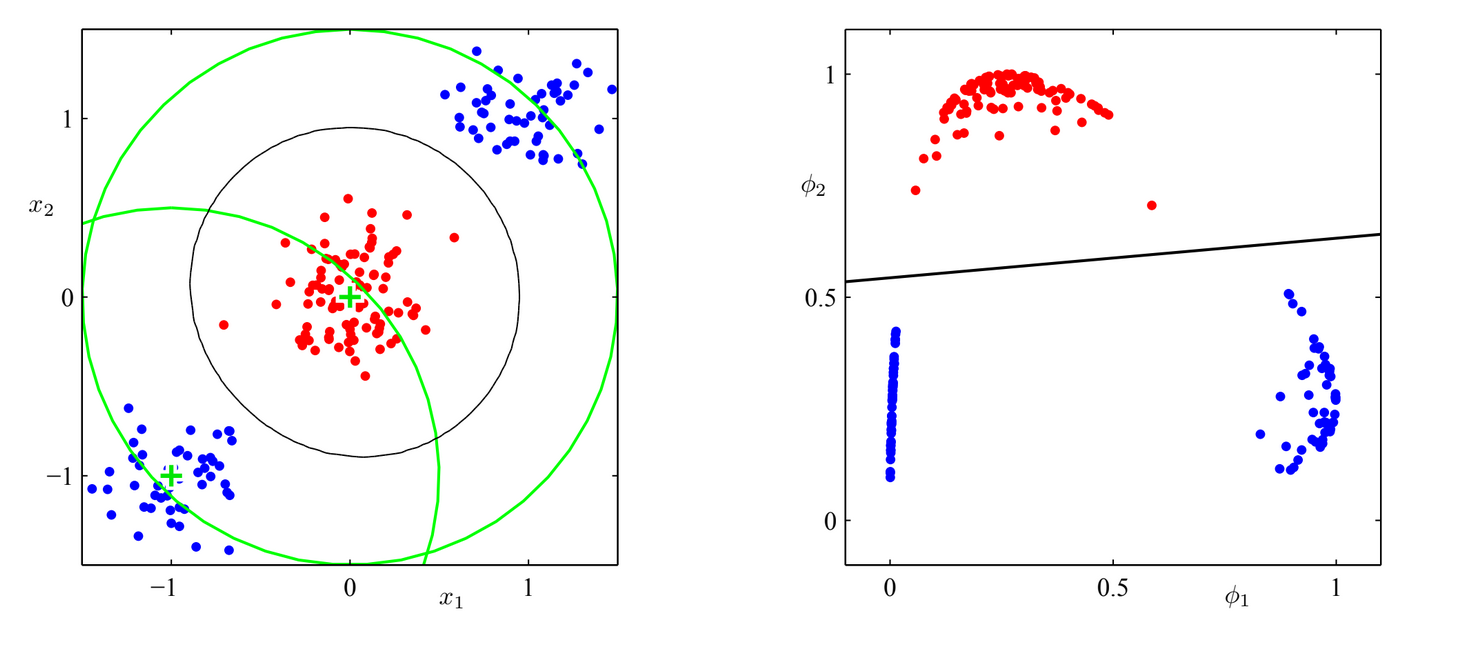
\includegraphics[width=15cm]{images/Probabilistic Models/phi_on_dataset.png}
    \caption{}
    \label{fig:phi_on_dataset}
\end{figure}

What we actually do is to train a linear model on a non-linear transformation:
\begin{equation}
    \begin{multlined}
    y(x) = w^{T}\phi(x) + w_{0} \text{    (two classes)} \\
    y_{k}(x) = w_{k}^{T}\phi(x) + w_{k0}\text{    (multiple\ classes)} \\
    \end{multlined}
\end{equation}
